% !TeX root = ../thuthesis-example.tex

\chapter{Introduction}
\label{chap:1}

Enzymes are proteins that catalyze biological reactions. They accelerate reactions 
to a speed that supports metabolic processes necessary for life. 
Understanding how enzymes work is crucial not only for grasping fundamental 
biological mechanisms but also for advancing medical science, 
particularly in the development of new pharmaceuticals and the engineering 
of enzymes with enhanced properties.

In order to design effective drugs or improve enzyme functions, 
one major challenge is the selection of the most promising compounds 
from a vast array of possibilities. 
Laboratory testing is costly and time-consuming. To reduce the possibilities,
using kinetic information can become a promising solution.

A key parameter in enzyme kinetics is the Michaelis constant ($K_m$). It represents
the substrate concentration at which the initial velocity of the reaction is half of
the maximum velocity. Generally, the lower the value, the higher is the affinity 
between the enzyme and the substrate.

Therefore, predicting the Michaelis constant can significantly accelerate the drug design process. 
By estimating an enzyme's affinity for various substrates and similarly, several enzymes
with one substrate, researchers can prioritize compounds for further development, 
thereby reducing the need for extensive laboratory testing. 
This approach not only facilitates the discovery of new drugs but also enhances 
our ability to engineer enzymes with desired characteristics.

\section{Problem statement}

The goal of this work is to build a statistical regression model that predict the 
Michaelis constant given 2 inputs: the protein sequence and the substrate string. 

The performance of the model will be evaluated with the mean squared error (MSE) and 
the coefficient of determination $r^2$.

\section{Literature review}

Given the interdisciplinary nature of this thesis, which involves biological, chemical, and 
computer sciences, the literature review will be structured in the following way.

First, the reader will be provided with the biological and chemical fundamentals necesarry to understand basic aspects
of enzyme kinetics. This foundation is essential to comprehend the biological processes at play and
their relevance to our work.

Second, machine learning and deep learning methodologies, emphasizing on their biological
applications, will be presented. This section aims to present how statistical models can be used to decipher complex biological
data, hence allowing us to build innovative solutions in enzyme and drug design.

Finally, a specific focus on the current state of research regarding the prediction of the Michaelis 
constant ($K_m$) will be offered. The aim of this part is to highlight the current contributions to 
our problem statement, the current state-of-the-art methods used, and their results.

Through this comprehensive review,the solid background provided will ensure the relevance of this thesis
contribution in the field of drug design.

\subsection{Biological and Chemistry Background}
\subsubsection{Proteins}
Proteins impact all the processes that take place in a cell, with an almost
endless diversity of functions. They are the most abundant biological macromolecules.
Thousands of different types of proteins can be found in a single cell. They are the molecular
instruments through which genetic information is expressed.\cite{lehninger}.

A protein is a sequence of smaller molecules called amino acids that are covalently joined by a peptide
bond. There exists 20 common amino acids (Figure \ref{fig:20aa}) from which almost all proteins are made of. Each amino acid has
a side chain with distinctive chemical properties.

\begin{figure}
  \centering
  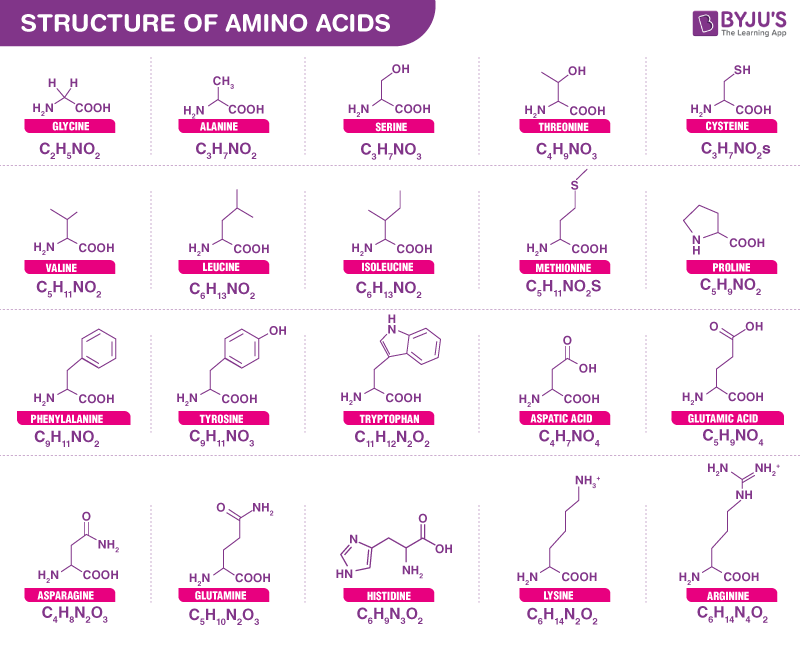
\includegraphics[width=0.7\linewidth]{1-amino_acids.png}
  \caption{The 20 common amino acids}
  % https://www.google.com.hk/url?sa=i&url=https%3A%2F%2Fbyjus.com%2Fbiology%2Famino-acids%2F&psig=AOvVaw1r9URV_-jl8bxr1TZ5ehjk&ust=1710296952635000&source=images&cd=vfe&opi=89978449&ved=0CBMQjRxqFwoTCIjpnuXW7YQDFQAAAAAdAAAAABAE
  \label{fig:20aa}
\end{figure}

All common amino acids are $\alpha$-amino acids. This means that both the carboxyl group and the amino group
is bonded to the same carbon atom called the $\alpha$-carbon (Figure \ref{fig:aastructure}). The amino acids differ from each others in
their side chains, also called R-groups, which vary in size, structure, electronic charge, and which
influence the solubility of the amino acids in water.

\begin{figure}
  \centering
  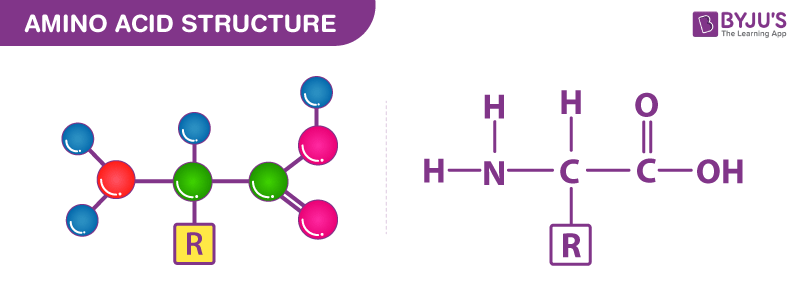
\includegraphics[width=0.3\linewidth]{1-amino_acid_structure.png}
  \caption{Amino acid structure}
  % https://www.google.com.hk/url?sa=i&url=https%3A%2F%2Fen.wikipedia.org%2Fwiki%2FAmino_acid&psig=AOvVaw1uUyMqtMb_u6DnLzN1XZTr&ust=1710297308181000&source=images&cd=vfe&opi=89978449&ved=0CBMQjRxqFwoTCOiroY7Y7YQDFQAAAAAdAAAAABAD
  \label{fig:aastructure}
\end{figure}

Two amino acids can be joined together with a covalent bond that is called a peptide bond. This link
is formed by the removal of the element of water (a hydroxyl group from the $\alpha$-carboxyl group
of one amino acid and a hydrogen atom from the $\alpha$-amino group of another amino acid. Figure 
\ref{fig:peptidebond}). These joined amino acids are called residues, relfecting the loss of the element
of water during the bonding formation.

\begin{figure}
  \centering
  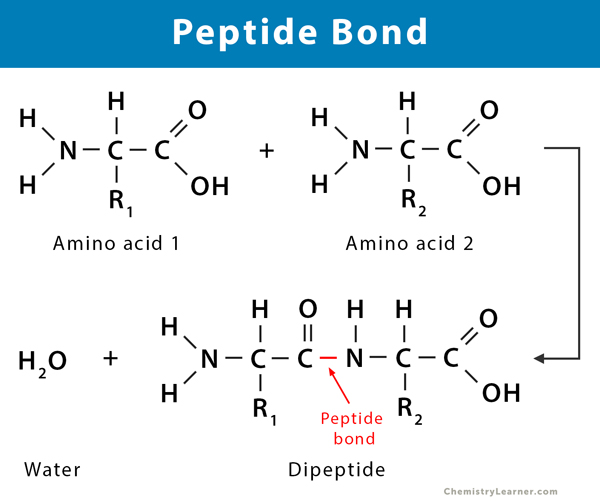
\includegraphics[width=0.5\linewidth]{1-peptide_bond.jpeg}
  \caption{Peptide bond}
  %https://www.chemistrylearner.com/wp-content/uploads/2020/10/Peptide-Bond.jpg
  \label{fig:peptidebond}
\end{figure}

An oligopeptide is the structure of a few amino acids joined together and a polypeptide is the name
given to the structure when many amino acids are joined. Proteins may have thousands of amino acids residues.

For proteins, the amino acid residues at the end are the $\alpha$-amino group called N-terminal and 
the $\alpha$-carboxyl group called C-terminal. The N-terminal is conventionally placed on the left while
the C-terminal is placed on the right.

The functions of proteins do not depend on their length or molecular weight. Some very small proteins 
(2 to 10 amino acids) can be extremely important such as toxic mushroom poisons or antibiotics (example + ref). The
length of proteins can vary enourmously from 2 to 27,000 amino acids, while the vast majority of proteins
usually contain fewer than 2,000 amino acids.

Some proteins are made of only one polypeptide chain while other can be made out of several, they are 
called mutlisubunit proteins, such as hemoglobin (example + ref).

Some proteins also contain chemical groups other than amino acids. They are called conjugated proteins.
The non-amino acid part of these proteins is called its prosthetic group and is essential to the protein
overall functions, such as hemoglobin and its ferrous group without which it does not function properly 
(check this + example + ref)

\subsubsection{Enzymes}
Enzymes are specific proteins that accelerate the rate of reactions. They are essential to life as many
of the chemical reactions essential to our survival need to be accelerated, such as the conversion of sugar.
(add example). 

\subsubsection{Pocket detection}
xxxx


\subsubsection{Substrates}
Substrates are the small molecules that interact with enzymes.

xxx
\subsubsection{Enzyme Kinetics}
kcat and Km

\subsection{Machine and Deep Learning for Drug Discovery}
\subsubsection{Traditional approaches}
\subsubsection{Machine Learning approaches}
\subsubsection{Neural Networks}
\subsubsection{Protein Language Models}
\subsubsection{Graph Neural Networks}

\subsection{Michaelis constant prediction}

Predicting the Michaelis constant represents a critical intersection of computational biology 
and enzymology, where the precise quantification of enzyme-substrate affinity becomes possible 
through advanced computational models. This section delves into the pivotal aspects of $K_m$
prediction, comprising the datasets used for model training and validation, 
the methodologies currently in practice, and an overview of the state-of-the-art performances achieved 
in this domain. 
\subsubsection{Dataset}
\label{sec:dataset}
The foundation of any computational approach to predicting the Michaelis constant is the dataset. 
This section describes the characteristics of the datasets employed, including the source of the 
protein and substrate sequences, the diversity of the enzyme classes represented, and the annotations of 
the Michaelis constant.

Before detailing the dataset preprocessing, it is essential to mention the elements it will be composed of.
The dataset will be made of 3 elements: protein sequences, a substrate string in SMILES format, and a
numerical $K_m$ value.

The SMILES (Simplified Molecular Input Line Entry System) notation is widely used method for 
representing the structure of chemical molecules using short ASCII strings. \cite{smiles}
Developed in the 1980s by Arthur Weininger and colleagues, SMILES has become a standard for the 
electronic storage of molecular information in databases and for the exchange of molecular structures 
between different software applications. It's particularly valued for its simplicity and the 
compactness of its representations, which allow for efficient processing and analysis of chemical 
structures by computers.

The key features of the SMILES notations are:
\begin{itemize}
  \item Atoms: Atoms are represented by their chemical symbol with hydrogen atoms usually 
  omitted (assumed implicitly). For example, the SMILES for ethanol (C2H5OH) is simply CCO, 
  implicitly understood as C2H6O.
  \item Bonds: Single bonds are not explicitly represented, while double, triple, 
  and aromatic bonds are denoted by =, \#, and :, respectively. For example, ethene (C2H4) 
  has the SMILES C=C.
  \item Branching: Branches are denoted by parentheses. For instance, isobutane (C4H10) can be 
  represented as CC(C)C.
  \item Rings: Ring structures are indicated by using numerical digits to represent the 
  connection point in a ring closure. For example, cyclohexane is represented as C1CCCCC1.
  \item Chirality: Chirality is specified using @ symbols. The @ symbol indicates one stereoisomer, 
  and @@ indicates the other.
\end{itemize}

Two databases using this notation are worth mentioning for to better understand the creation of the dataset:
KEGG and PubChem. \cite{kegg,pubmec} The Kyoto Encyclopedia of Genes and Genomes (KEGG) is a 
comprehensive database integrating genomic, chemical, and systemic functional information. 
It offers resources for the systematic analysis of gene functions in terms of the networks of 
genes and molecules. KEGG facilitates understanding of biological processes and their underlying 
mechanisms by categorizing gene products into their respective pathways and modules, providing a 
platform for both bioinformatics and systems biology. It possesses a unique way to identify all molecular
compounds called KEGG ID.
PubChem, on the other hand, is a database of chemical molecules and their activities 
against biological assays. Operated by the National Center for Biotechnology Information (NCBI), 
it is a vital resource for chemists, biochemists, and biologists. 
PubChem contains information on the chemical structure, identification, biological activities, 
patents, and literature citations of compounds. It supports the search for chemical substances 
by name, molecular formula, structure, and other identifiers, making it an invaluable tool for 
researchers in drug discovery and pharmacology. It also possesses a unique way to identify all molecular
compounds called PubChem ID.

The dataset used is obtained from \citeauthor{km1} as it is the standard dataset used for the most recent Michaelis
constant prediction models. It is comprised of 11,675 enzyme-substrate pairs and their associated $K_m$ value in
the format defined above: protein sequences, substrate strings in SMILES format, and numerical $K_m$ values
that have been log10 transform as the Michaelis constant values usually range from $10^{-1}$ to  $10^{-7}$.

The 11,675 entries of the dataset were compiled from the BRENDA database. \cite{brenda} The BRENDA 
(BRaunschweig ENzyme DAtabase) database is a comprehensive collection of 
enzyme and metabolic information, widely recognized as one of the most detailed 
and user-friendly resources for enzyme data. It was initially developed at the Technical 
University of Braunschweig, Germany, and has been continuously updated and expanded since its 
inception in the 1980s. BRENDA offers an extensive range of data on enzyme function, 
classification, kinetics, and molecular properties, making it an invaluable tool for 
researchers in biochemistry, molecular biology, and related fields.

At the time of the dataset creation, 156,387 entries detailing $K_m$ values, organism and substrate names, 
EC numbers, UniProt IDs of enzymes, and PubMed IDs. To enhance data specificity and compatibility, 
substrate names were aligned with KEGG Compound IDs using KEGG and PubChem synonym lists. \cite{kegg}
When necessary, PubChem IDs were mapped to KEGG IDs via MBROLE's web service. \cite{pubchem,mbrole}
Amino acid sequences were acquired through UniProt's mapping service if they were available. \cite{uniprot}
When the UniProt ID was not available, the sequence was directly retrived from BRENDA by selecting a
sequence with the same EC Number and organism. The dataset was then processed to eliminate duplicates, 
non-wild-type enzymes, 
entries from nonbacterial organisms lacking UniProt IDs, and substrates unidentifiable with KEGG IDs, 
adding up to 34,526 entries. Only entries with natural substrates were keep, 
as indicated by their presence in the KEGG reaction database, resulting in 11,675 viable data points. 
These entries were log10-transformed for consistency, with the dataset randomly divided into training 
(70\%), validation (10\%), and test (20\%) sets. 

This dataset is the most commonly used for Michaelis constant prediction. 

\subsubsection{Current Methods}

As of today, 4 models offer the best performances for predicting the Michaelis constant on the dataset
at hand. In this section, we delve into each of them.

The first model we will discuss is by the authors of the dataset themselves, \citeauthor{km1} as they were
the frist one to curate a dataset for this task and built a model for it. They offer a method using both
Machine and Deep Learning. For the substrate, it is represented as a molecular graph based on its atoms and
bonds. This information can be extracted from the SMILES representation using RDKit. \cite{rdkit} They are
then processed by a Graph Convolutional Neural Network to produce an embedding for each substrate. This 
embedding is then concatenated to a UniRep embedding of the protein sequence. \cite{unirep} 
Then, this new vector is fed into a gradient boosting model, XGBoost. \cite{xgboost}

Another model called ENKIE (ENzyme KInetics Estimator) uses hierarchical Bayesian Multilevel
Models to predict value and uncertainty of the Michaelis constant. In this paper, the assumption is that
the residuals are normally distributed, defined by means ($\mu_*$) and standard deviations ($\sigma_*$), 
accounting for the inherent variability in enzyme behavior without directly addressing 
the structural and physical complexity of the enzymes and their interactions. It categorizes data based on
substrates which introduces group-level effects that reflect the nested nature of 
biological processes. Hence, the protein sequence is not directly used but instead information about the
protein such as EC Number, protein family, and UniProt ID. Are also used reaction stoichiometries and
identifiers, as well as optionally physiological properties of the reaction compartments (pH, pMg, 
temperature and ionic strength).

\begin{figure}
  \centering
  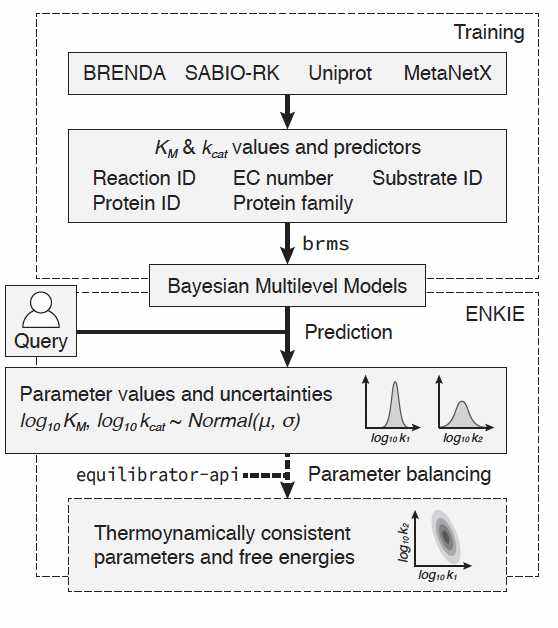
\includegraphics[width=0.5\linewidth]{1-enkie.png}
  \caption{ENKIE model overview}
  \label{fig:enkie}
\end{figure}

Published in Nature Communications, UniKP is a unified framework based on pretrained large language models
for predicting enzyme kinetic parameters: the enzyme turnover number ($k_{cat}$), the Michaelis constant
($K_m$), and the catalytic efficiency ($\frac{k_{cat}}{K_m}$). Similarly to \citeauthor{km1} is uses both the
protein sequence and the substrate string. It is comprised of 2 main components : a representation module 
for both the protein sequence (Figure \ref{fig:unikp}, part a) and the substrate string 
(Figure \ref{fig:unikp}, part b) and a machine learning module (Figure \ref{fig:unikp}, part c). 
Part d on Figure \ref{fig:unikp} are only relevent for $k_{cat}$ and include additional features into the model
such as pH and temperature. Part e of Figure \ref{fig:unikp} represents the re-weighting methods used 
to adjust the sample weight distribution to generate an optimized prediction. For the protein, the ProtT5-XL
model is used where, for each sequence, each amino acid is turned into a 1024-dimensional vector. To obtain
a condensed representation for each protein, mean pooling is applied. For the substrate, it is processed in
a similar way where each character of the string is processed by the SMILES-Transformer, resulting in a 
256-dimensional vector for each symbol. To get an equivalent 1024-dimensional vector for the substrate,
mean and max pooling are applied to these vectors and concatenated with the first and last output of the
model, as they are the start (SOS) and end of sequence (EOS). Then, both the protein and substrate representations
are contatenated and fed into the machine learning module. The latter is Extremely Randomized Trees, an
ensemble method that combines the predictions of multiple de-correlated decision trees to make more 
accurate and stable predictions than any single decision tree. It is similar to Random Forests but 
introduces extra randomness in the way splits are made at the nodes of the decision trees. \cite{extratrees}

\begin{figure}
  \centering
  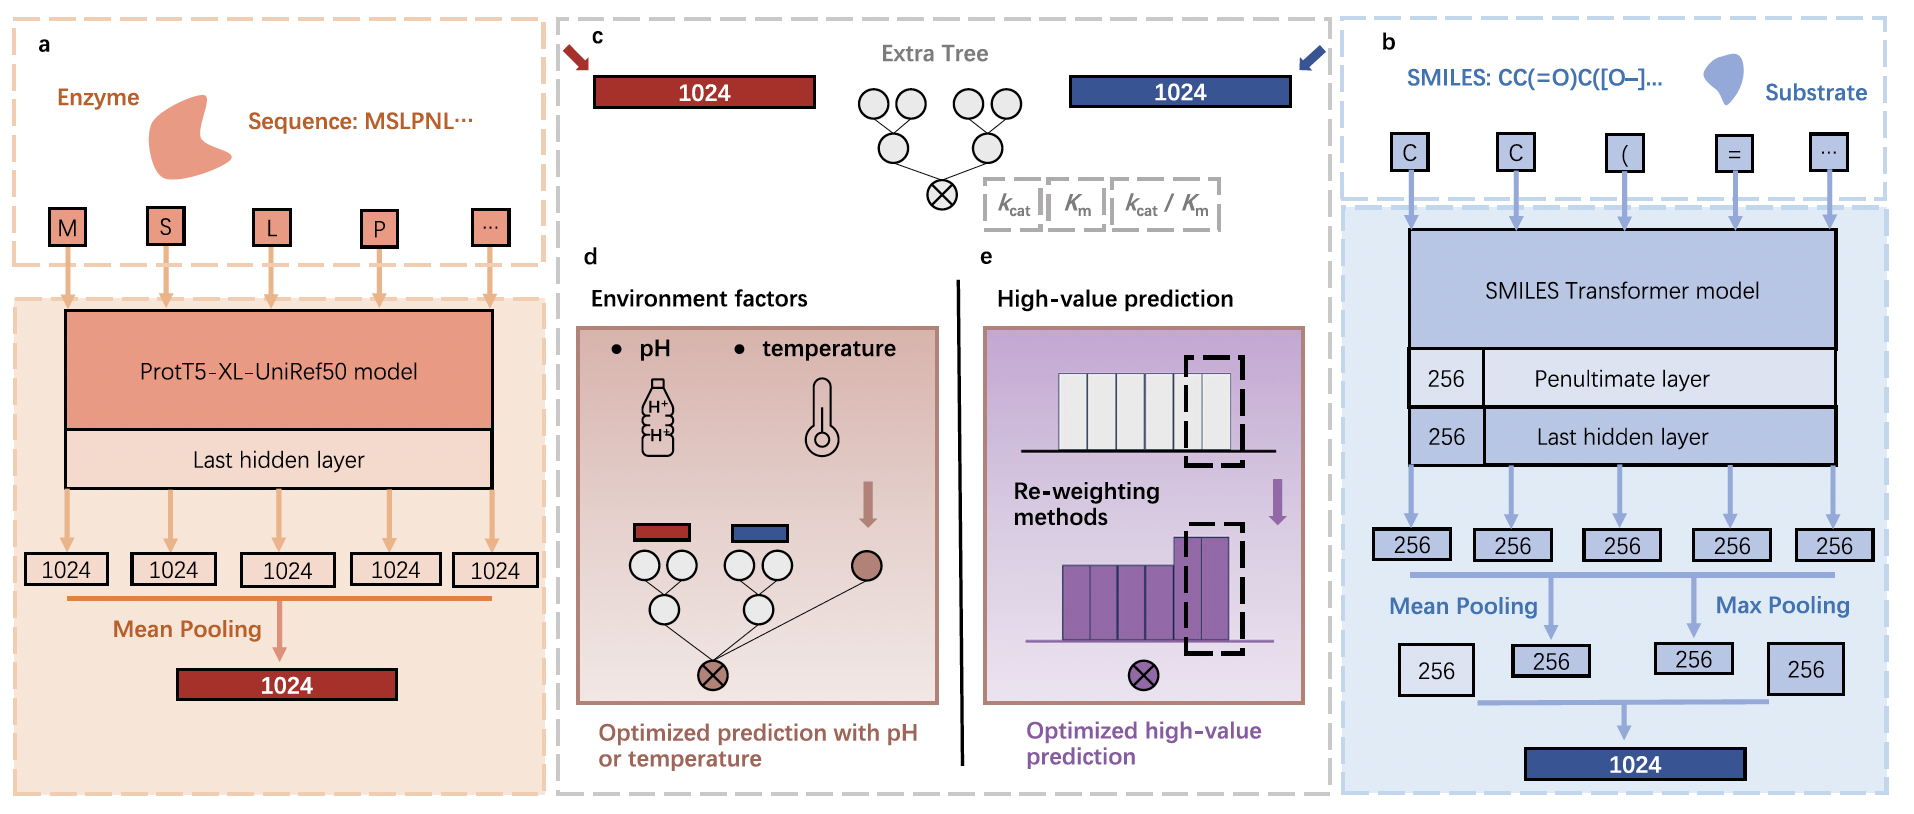
\includegraphics[width=1\linewidth]{1-unikp.png}
  \caption{UniKP model overview}
  \label{fig:unikp}
\end{figure}

Finally, the last method we will present is ProSmith. \cite{prosmith} While it hasn't been published yet
and is only available in preprint, it offers the best results for this task. This model employs a multimodal
transformer network to simultaneously process protein amino acid sequences and substrate strings. To do so,
the model use a concatenation approach where the protein sequence and substrate string are concatenated 
and separated by a separation token. In order to process this input, the network divide it into chunk 
known as tokens. For protein sequences, the tokens are the amino acids and for substrate, each symbol is
treated as a separate token. ProSmith use pre-learned token representations that were trained independently
on each modality. For amino acid representations, ESM-1b model was used and for the SMILES string tokens, it
was ChemBERTa2. \cite{esm1,chemberta} The token embeddings from ESM-1b and ChemBERTa2 have different dimensions,
1280 and 600 respectively. To process them using the same transformer network, the authors used linear layers
to map both sets of embeddings to a joint embedding space with a dimension of 768, which is also the hidden
dimension of all tokens in the ProSmith transformer network. 

\begin{figure}
  \centering
  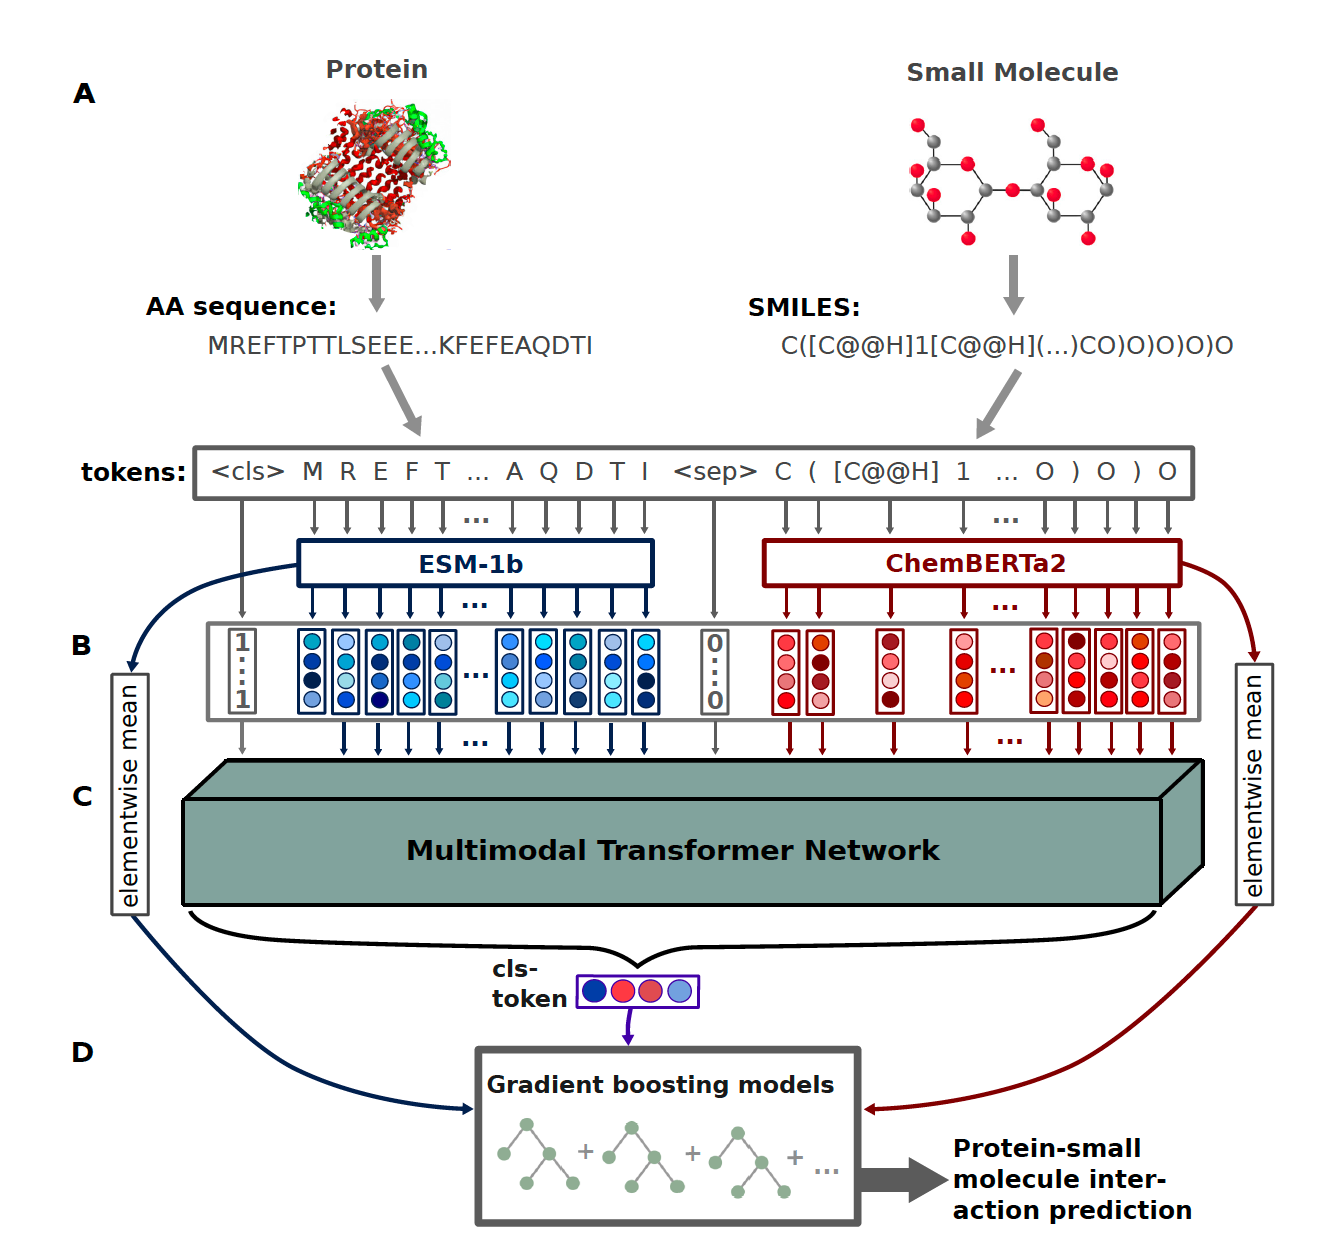
\includegraphics[width=1\linewidth]{1-prosmith.png}
  \caption{ProSmith model overview}
  \label{fig:prosmith}
\end{figure}

During the processing steps, the transformer 
network updates each input token using the attention mechanism, with 6 attention layers, each having
6 attention heads. \cite{attention} This enables the model
to look at the entire input sequence and selectly focus only on relevant token for making updates. 
After the update of all input tokens for a predefined number of steps, the classification token cls is
extracted and used as the input for a fully connected neural network, which is trained to predict an
interaction between the enzyme and the substrate. Then, the cls token, along with the original protein 
embedding from ESM-1b and substrate embedding from ChemBERTa2 are used as input to a gradient boosting model.
\cite{xgboost} This transformer model was pretrained on the Ligand-Target-Affinity Dataset from BindingDB.
\cite{bindingdb} All drug-target pairs with experimentally measured IC50 values were extracted and pairs 
that would be used for evaluation were removed. This results in 1,039,565 entries for the dataset. 95\%
were used for training ang 5\% for validation. The transformer network was trained for 100 epochs and saved
after each one. The model with the best results on the validation set was selected. Finally, the model
was fine-tuned for different tasks including the Michaelis constant on the dataset we discussed in this 
chapter.

The model presented in the previous section have the following results:

\begin{table}[ht]
  \centering
  \begin{tabular}{lcc}
    \hline
    Method & MSE \(\downarrow\) & \(R^2\) \(\uparrow\) \\
    \hline
    ENKIE (2022) & -- & 0.463 \\
    Kroll et al. (2021) & 0.653 & 0.527 \\
    UniKP (2023) & 0.640 & 0.530 \\
    ProSmith (2023) & 0.604 & 0.563 \\
    \hline
  \end{tabular}
  \caption{Comparison of model performance for $K_m$ prediction}
  \label{tab:model_performance}
\end{table}


\section{Methodology}
This research will be composed of a data preprocessing step, a model implementation step, and an
evaluation step. Python 3.9 and PyTorch 2.0.1 will be used for these steps.

\subsection{Data preprocessing}
In this work, we will use the dataset prepared by \citeauthor{km1} and presented in the section \ref{sec:dataset}
The data used is up to 2022. Therefore, we will augment their dataset with a new test set composed of
the data from 2022 to January 2024, allowing a better testing of the current methods and the validation
of this work.
For all our model, we will therefore compute the metrics on the test set provided by the original dataset,
as well as on our new test dataset.
The processing of the new test set will be the same as for the original dataset.

\subsection{Model implementation}
The model implementation will be composed of 3 parts. The first one will be the creation of an architecture
for the sequence-based model, the for the structure-based model, and finally for the ensemble model using both
the sequence-based and the structure-based model.

\subsection{Model evaluation}
The 3 models of this work (sequence-based model, structure-based model, and sequence-structure-based model)
will be evaluated on the ProSmith test set as well as our newly curated test set. The evaluation metrics 
wil be the mean squared error (MSE) and the coefficient of determination $r^2$.

Not only will this work evaluate these metrics in the general sense but it will also provide a more specific
set of these metrics based on the data: the protein sequences and the substrates strings will be divided into
4 groups based on their appearance in the training set. Proteins that have been seen in the training set
will be denoted "hot proteins" and the ones that are not in the training set "cold proteins". Similarly, 
subrates included in the training set will be denoted "hot substrates" and "cold substrates" if they
are not.

These 4 groups will allow a better comparison of this work method and the state-of-the-art methods.

